\documentclass[fleqn,10pt]{olplainarticle}
% Use option lineno for line numbers 

\title{Conditional Probabilistic Anatomical Reasoning for Pan-Cancer Multi-Agent Tumor Segmentation and Analysis}

\author[1]{First Author}
\author[2]{Second Author}
\affil[1]{Address of first author}
\affil[2]{Address of second author}

\keywords{Keyword1, Keyword2, Keyword3}

\begin{abstract}
Please provide an abstract of no more than 300 words. Your abstract should explain the main contributions of your article, and should not contain any material that is not included in the main text. 
\end{abstract}

\begin{document}

\flushbottom
\maketitle
\thispagestyle{empty}

\section{Introduction}

\begin{itemize}
    \item Build a pan-cancer multi-agent tumor segmentation system
    \item 2D, 3D tumor segmentation models, anatomical segmentation models could be any, even allow users to define or use their private models
    \item Beyond segmentation, provide anatomical graph and explanation
\end{itemize}

\section{Methodology}
\begin{figure*}[t]
    \centering
    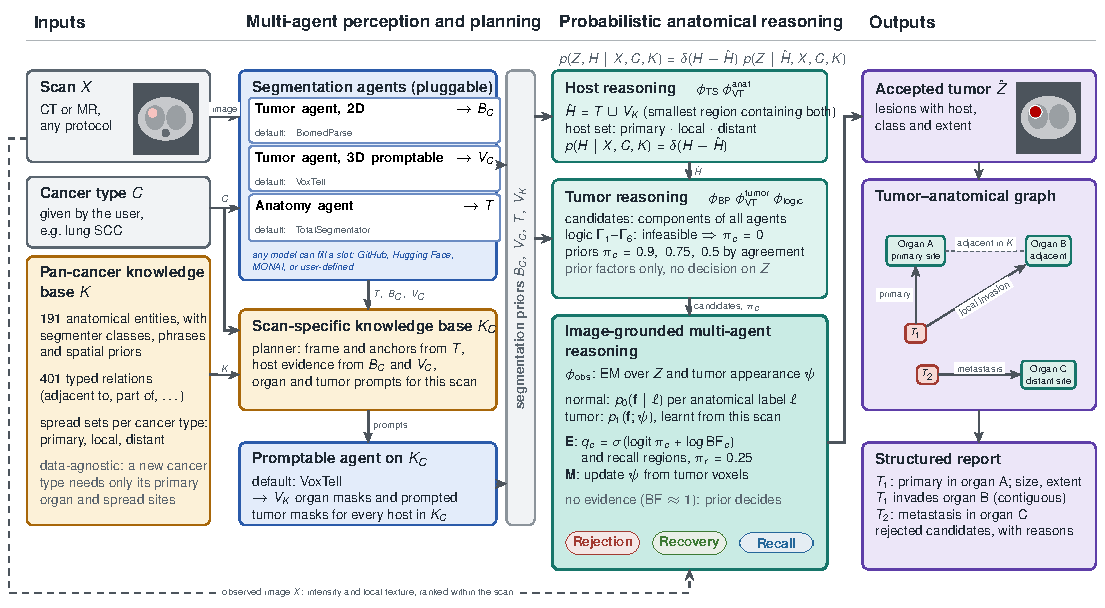
\includegraphics[width=\linewidth]{figs/pipeline.pdf}
    \caption{Pan-cancer multi-agent tumor segmentation and reasoning. Given a scan $X$ and a user-given cancer type $C$,
    pluggable segmentation agents (defaults: BiomedParse for 2D tumor, VoxTell for 3D promptable tumor and anatomy,
    TotalSegmentator for anatomy; any model from GitHub, Hugging Face, MONAI or a user can fill a slot) produce tumor
    priors $B_C,V_C$ and anatomy $T$. A planner turns the pan-cancer knowledge base $K$ into a scan-specific plan $K_C$,
    which a promptable agent executes to give organ masks $V_K$ and prompted tumor masks. Host reasoning fixes the host
    $\hat H$; tumor reasoning evaluates the prior factors of every candidate (logical feasibility and agreement), without
    deciding the tumor; image-grounded reasoning then infers the tumor posterior by EM against label-conditional normal
    tissue models and a scan-specific tumor model, which rejects, recovers and recalls tumor tissue. The accepted tumor is
    organized into a tumor--anatomical graph and a structured report.}
    \label{fig:pipeline}
\end{figure*}

Figure~\ref{fig:pipeline} summarizes the pipeline; the components are detailed below.

\subsection{Conditional Probabilistic Anatomical Reasoning}
\label{sec:conditional_reasoning}
\begin{figure}
    \centering
    \includegraphics[width=1\linewidth]{figs/PGM.png}
    \caption{ Anatomical Reasoning Graph.}
    \label{fig:pgm}
\end{figure}

We formulate tumor segmentation as a conditional
probabilistic anatomical reasoning problem that
jointly infers tumors and their host anatomical
structures by integrating image-dependent
segmentation priors with anatomical and
logical constraints.
Let $X$ denote the observed medical image,
$Z$ denote the tumor segmentation, and $H$
denote the host anatomical segmentation.
We further denote the cancer type by $C$
and the data-agnostic anatomical knowledge
base by $K$.
Our framework consists of three complementary
components: (1) observation consistency,
(2) tumor reasoning, and (3) host reasoning.

\paragraph{Image-Dependent Segmentation Priors.}

We construct four complementary segmentation
priors to provide image-dependent evidence
for tumor and host anatomical reasoning.

For tumor reasoning, we employ cancer-type
prompting to obtain 2D and 3D tumor
segmentation priors from BP and VT,
respectively:
\begin{equation}
\label{eq:tumor_priors}
\begin{aligned}
B_C &= f_{\mathrm{BP}}(X,C),\\
V_C &= f_{\mathrm{VT}}(X,C),
\end{aligned}
\end{equation}
where $B_C$ provides slice-wise tumor
segmentation evidence and $V_C$ provides
volumetric tumor segmentation evidence.

For host reasoning, we obtain two complementary
anatomical segmentation priors.
First, the data-agnostic anatomical
knowledge base $K$ is specialized to the scan
as a prompt plan $K_C$ (Section~\ref{sec:kb_planning}),
which VT executes, yielding a cancer-specific
anatomical segmentation prior:
\begin{equation}
\label{eq:kb_prior}
V_K = f_{\mathrm{VT}}(X,K_C).
\end{equation}
Second, we employ TotalSegmentator to
generate a cancer-agnostic anatomical segmentation
prior without explicit prompting:
\begin{equation}
\label{eq:ts_prior}
T = f_{\mathrm{TS}}(X).
\end{equation}
Although the anatomical knowledge base itself
is independent of the observed image, the
corresponding VT segmentation output $V_K$
is image-dependent.
The tumor prompts of $K_C$ yield further VT tumor
masks, one per host of the cancer type, which are
included in $V_C$ as candidates.
Consequently, the framework incorporates
two tumor segmentation priors,
$\{B_C,V_C\}$, and two host anatomical
segmentation priors, $\{V_K,T\}$.

\paragraph{Conditional Probabilistic Formulation.}

Given the observed image, cancer type,
and anatomical knowledge base, we model
the joint conditional distribution of
tumor and host segmentations in a
modular form,
\begin{equation}
\label{eq:conditional_joint}
\boxed{
p(Z,H\mid X,C,K)
=
p(H\mid X,C,K)\;
p(Z\mid H,X,C,K)
}
\end{equation}
with a host model and a tumor model given the host,
\begin{equation}
\label{eq:reasoning_potentials}
\begin{aligned}
p(H\mid X,C,K)
&\propto
\phi_{\mathrm{host}}(H;V_K,T),\\
p(Z\mid H,X,C,K)
&=
\frac{1}{\mathcal{Z}(H,X,C,K)}\,
\phi_{\mathrm{obs}}(Z,H;X)\,
\phi_{\mathrm{tumor}}(Z,H;B_C,V_C),
\end{aligned}
\end{equation}
where $\mathcal{Z}(H,X,C,K)$ normalizes
the tumor model separately for every host
configuration.
The host model depends on the image through the
anatomical priors $T$ and $V_K$, and the tumor model
depends on it through the tumor priors $B_C$, $V_C$
and the observation potential.

Equation~\eqref{eq:conditional_joint} differs from a
single jointly normalized product of the three
potentials in one respect: evidence about the tumor
does not feed back into the host. This is a
\emph{cut} or modular formulation of a
graphical model~\cite{liu2009modularization,plummer2015cuts,jacob2017better},
used when one module is more reliable than another
and feedback would let the less reliable one corrupt
it. Here the anatomical priors are more reliable than
the tumor priors, and feedback would allow uncertain
tumor candidates to reshape the anatomy, for example
by enlarging an organ until a false-positive candidate
becomes anatomically feasible.
This conditional formulation directly
incorporates the image-dependent segmentation
priors without assuming that they are
independent of the observed image or
constitute data-independent Bayesian priors.

\paragraph{Host Reasoning.}

The host potential integrates
two complementary sources of image-dependent
anatomical evidence: the KB-prompted VT
segmentation prior and the non-prompted
TotalSegmentator segmentation prior,
\begin{equation}
\label{eq:host_reasoning}
\phi_{\mathrm{host}}(H;V_K,T)
=\phi_{\mathrm{VT}}^{\mathrm{anat}}(H;V_K)\cdot
\phi_{\mathrm{TS}}(H;T).
\end{equation}
The KB-prompted VT potential incorporates
patient-specific anatomical evidence
obtained through knowledge-guided
segmentation, whereas the TotalSegmentator
potential provides complementary anatomical
evidence without explicit prompting.
Both act as containment constraints: each host
region must contain the anatomy delineated by either
prior. We take the host model to be deterministic,
\begin{equation}
\label{eq:host_point_mass}
p(H\mid X,C,K)=\delta\bigl(H-\hat H\bigr),
\end{equation}
where $\hat H$ is the smallest configuration that
satisfies both constraints
(Section~\ref{sec:reasoning_details}); that is, the host
is a deterministic function of the image-dependent
anatomical priors.
A cancer sits in its primary site with high prior but may have invaded neighbours or spread, so the host is a set with weights, not one organ.

\paragraph{Tumor Reasoning.}

The tumor reasoning potential integrates
the cancer-type-prompted 2D and 3D tumor
segmentation priors with the inferred
host anatomical structures.
We formulate tumor reasoning through
set-theoretic operations and logical
constraints:
\begin{equation}
\label{eq:tumor_reasoning}
\begin{aligned}
\phi_{\mathrm{tumor}}
&(Z,H;B_C,V_C) =
\phi_{\mathrm{BP}}(Z;B_C)
\phi_{\mathrm{VT}}^{\mathrm{tumor}}(Z;V_C)
\phi_{\mathrm{logic}}(Z,H).
\end{aligned}
\end{equation}
The components of the 2D and 3D tumor priors are the
tumor candidates. The segmentation potentials
$\phi_{\mathrm{BP}}$ and $\phi_{\mathrm{VT}}^{\mathrm{tumor}}$
jointly assign each candidate a prior probability of being
tumor, according to whether the other model supports it.
The logical potential $\phi_{\mathrm{logic}}$ encodes
anatomical relationships between tumors
and their host structures:
set-theoretic relations
such as containment, intersection,
and exclusion remove anatomically
implausible candidates.
The tumor potential thus acts as a prior over $Z$ given
the host; it is not yet the posterior.
Tumor reasoning does not optimize $Z$: it evaluates the
factors of the tumor model that do not involve the observation
likelihood (which candidates
exist, which are anatomically infeasible, and how probable each
is a priori) and does not select a tumor configuration while
ignoring the observation likelihood.
Its output initializes the tumor posterior; the tumor itself is
inferred only when these factors are combined with the
observation potential (Eq.~\eqref{eq:log_inference}).

\paragraph{Observation Consistency.}

The observation consistency potential
evaluates whether a hypothesized tumor
configuration is compatible with the
observed image. We employ statistical rejection to suppress
candidates that are inconsistent
with the observed image, \textbf{while statistical recall discovers additional tumor tissue that is consistent with the accepted tumor characteristics}.
Specifically, we define
\begin{equation}
\label{eq:observation_potential}
\phi_{\mathrm{obs}}(Z,H;X,\psi)
=
\exp\left[
-\lambda_{\mathrm{obs}}
E_{\mathrm{obs}}(Z,H;X,\psi)
\right],
\end{equation}
where $E_{\mathrm{obs}}$ is a
statistical inconsistency score comparing a normal-tissue
model of each anatomical structure with a tumor appearance
model $\psi$ (Section~\ref{sec:reasoning_details}), and
$\lambda_{\mathrm{obs}}$ controls the
strength of observation consistency.
The tumor appearance $\psi$ is specific to each scan and
unknown, so it is estimated jointly with the tumor
segmentation.

\paragraph{Joint Tumor--Host Inference.}

Substituting Eqs.~\eqref{eq:host_reasoning}--\eqref{eq:observation_potential}
into Eq.~\eqref{eq:conditional_joint}, the complete
conditional reasoning model is
\begin{equation}
\label{eq:expanded_reasoning}
\boxed{
\begin{aligned}
p(Z,H\mid X,C,K,\psi)
=\;&\delta\bigl(H-\hat H\bigr)\cdot
\frac{1}{\mathcal{Z}(H,X,C,K,\psi)}\,
\phi_{\mathrm{obs}}(Z,H;X,\psi) \\
&\cdot\phi_{\mathrm{BP}}(Z;B_C) \cdot\phi_{\mathrm{VT}}^{\mathrm{tumor}}
(Z;V_C) \cdot\phi_{\mathrm{logic}}(Z,H),
\end{aligned}
}
\end{equation}
with $\hat H$ determined by
$\phi_{\mathrm{VT}}^{\mathrm{anat}}(H;V_K)\,\phi_{\mathrm{TS}}(H;T)$.
The tumor and host segmentations are estimated by
maximum a posteriori inference,
\begin{equation}
\label{eq:map_inference}
(\hat Z,\hat H)
=
\arg\max_{Z,H}\;
p(Z,H\mid X,C,K,\psi).
\end{equation}
Because the host model is a point mass, every
configuration with $H\neq\hat H$ has zero probability,
and the joint maximum is attained at $H=\hat H$.
The MAP problem therefore reduces exactly to host
reasoning followed by tumor inference given the host.
The tumor appearance $\psi$ is a parameter of the observation
model, not a segmentation, so it is estimated by maximizing the
marginal likelihood over the candidate labels, and the labels
are then the MAP configuration given that estimate,
\begin{equation}
\label{eq:log_inference}
\begin{aligned}
\hat\psi&=\arg\max_{\psi}\;\log\sum_{Z}
\phi_{\mathrm{obs}}(Z,\hat H;X,\psi)\,\phi_{\mathrm{tumor}}(Z,\hat H;B_C,V_C),\\
\hat Z&=\arg\max_{Z}\;
\log\phi_{\mathrm{obs}}(Z,\hat H;X,\hat\psi)
+\log\phi_{\mathrm{tumor}}(Z,\hat H;B_C,V_C).
\end{aligned}
\end{equation}
The first problem is solved by expectation--maximization over the
candidate labels and $\psi$ (Section~\ref{sec:reasoning_details}),
whose E-step yields the posteriors from which $\hat Z$ follows.
Because the observation evidence is calibrated and the update is
damped, the procedure is a generalized EM without a monotonicity
guarantee; its convergence is verified empirically.
Statistical rejection, recovery and recall are outcomes of
this single inference.
Relaxing the cut, so that tumor evidence also refines the
host, would turn the procedure into block-coordinate
ascent over $(Z,H)$; we do not pursue this.
By integrating complementary tumor
segmentation priors, knowledge-guided
and non-prompted anatomical priors,
and explicit anatomical constraints,
the proposed framework enables
conditional probabilistic reasoning
over tumor--host configurations
under uncertainty.

\subsection{Pan-cancer knowledge base and prompt planning}
\label{sec:kb_planning}
% Drafted 4 Oct 2026 from knowledge base v0.5.7 (knowledge_base/*.yaml) and the planner (pancia_kb/planner.py,
% adapter.py). No equation of Section~\ref{sec:conditional_reasoning} is changed; this section defines how $K$ is
% built and how the prompt plan $K_C$ of Eq.~\eqref{eq:kb_prior} is produced for each scan.

This section describes how the anatomical knowledge base $K$ is built once for all cancer types, and how, for each scan,
it is turned into the final VT prompt plan $K_C$ of Eq.~\eqref{eq:kb_prior}. $K$ is a curated, image-independent graph;
$K_C$ is a finite list of prompt jobs, and $V_K=f_{\mathrm{VT}}(X,K_C)$ is the stack of masks VT returns for these jobs.
No component of $K$ or of the planner uses patient sex, and no rule or constant is specific to an organ, a cancer type
or a dataset.

\paragraph{Anatomical entities.}
$K$ contains 204 anatomical entities. Each entity has a category (solid organ, hollow organ, gland, bone, vessel,
lymph-node station, muscle, fascia, fat, duct, space, nerve, landmark or region) and a laterality (left, right, midline
or bilateral). It also records how it can be observed: the TotalSegmentator classes that represent it for CT and for
MR, if any; a VT main phrase with up to two aliases, each graded as in-vocabulary, near-vocabulary or
out-of-vocabulary against the published VT training vocabulary; its craniocaudal span between vertebral anchors;
whether it is always present, variably present or absent after common surgery; a typical volume range; and, for CT, a
typical Hounsfield-unit range. Finally, each entity that can host a tumor carries a tumor phrase (for example
\emph{liver tumor}). Thirty-nine entities are \emph{anchors}: structures that TotalSegmentator segments reliably and
that therefore fix the coordinate frame of a scan (vertebrae, major vessels and large organs). Landmarks are tied to
vertebral levels, so that every spatial prior in $K$ is expressed relative to the patient's own skeleton rather than in
millimetres.

\paragraph{Anatomical relations.}
Entities are connected by 433 typed, directed relations. Ten relation kinds are defined, of which nine are used:
\emph{adjacent\_to} (176), \emph{has\_part} (97), \emph{drains\_lymph\_to} (62), \emph{lies\_in} (23),
\emph{supplied\_by} (21), \emph{invested\_by} (16), \emph{drained\_by} (16), \emph{landmark\_for} (13) and
\emph{has\_duct} (9); the tenth, \emph{wall\_of}, is reserved. Each relation kind has a fixed spatial gate and a default
priority. The gate states where the target may lie relative to the source: inside it (\emph{has\_part}), in a shell
around it (\emph{invested\_by}), in a neighbouring box or directional shell (\emph{adjacent\_to}), in a corridor along
a vessel or duct (\emph{supplied\_by}, \emph{drained\_by}, \emph{has\_duct}) or in a body region
(\emph{drains\_lymph\_to}); \emph{lies\_in} and \emph{landmark\_for} carry no gate. Gates are later used to check VT
outputs against structures that are already segmented, and priorities order prompts when the budget is exceeded. The relations encode the anatomy that staging systems refer to: direct extension
into a neighbouring organ, invasion of an investing fascia or fat, and lymphatic drainage to a regional station.

\paragraph{Cancer-type spread sets.}
For each cancer type $C$, $K$ stores a weighted host set $\mathcal{H}_C$, which is the host set used in
Section~\ref{sec:reasoning_details}. Only two items are specified per cancer type: the primary organ (prior $1.0$) and a list of
distant metastatic sites (prior $0.15$). Organs at risk of local invasion (prior $0.3$) are not curated; they are
derived automatically as the entities reached from the primary organ by an \emph{adjacent\_to} or \emph{invested\_by}
relation. Each cancer type also has a short ensemble of tumor phrases (for example \emph{lung cancer}, \emph{lung
tumor}, \emph{lung mass}), and generic templates produce phrases for any host without a curated one. The distant-site lists are user-defined inputs rather than an exhaustive account of metastatic spread. Here we
restrict each list to the most common metastatic sites reported for that cancer type that are also anchors of $K$, and
cancer types without a curated list default to liver, lung, adrenal gland and spine. Head-and-neck anchors (brain, oral cavity,
pharynx, larynx and parotid gland) are part of $K$ but are in no default list, because the body scans considered here
rarely include the head and neck. Sites that are not anchors, such
as the pleura and distant lymph nodes, are not prompted. A user can extend a list, or add an anchor, without changing any other part of the framework, and only the affected cancer types need to be re-planned. The current
base covers 17 TCGA cancer types, plus a CPTAC entry whose cancer type is resolved per case. Adding a new cancer type
therefore requires only its primary organ, its metastatic sites and, optionally, its phrase ensemble; all other
knowledge is shared.

\paragraph{Planning $K_C$ for a scan.}
For a given scan, the planner builds $K_C$ deterministically in a single pass, without calling any segmentation model.
Its inputs are the modality, the cancer type $C$, a summary of the TotalSegmentator output $T$ (which classes are
present, their volumes and their extents), and the initial tumor priors $B_C$ and $V_C$ of Eq.~\eqref{eq:tumor_priors}.
It proceeds in five steps.

\emph{(i) Frame.} The vertebrae found in $T$ define a craniocaudal ruler. The landmarks of $K$ are placed on this ruler,
and every entity span is converted to a slice range of the scan. This step also determines which entities lie inside the
field of view.

\emph{(ii) Anchors.} Each anchor is labelled \emph{found} (present in $T$ with a plausible volume and position),
\emph{expected} (inside the field of view but missing from $T$) or \emph{missing} (outside the field of view). Found
anchors give the reference structures against which the gates of later prompts are evaluated.

\emph{(iii) Tumor evidence.} A component of $B_C$ or $V_C$ is \emph{validated} when the two priors agree on it. For each
host $h\in\mathcal{H}_C$ the planner records an evidence level $e_h\in\{0,1,2\}$: $2$ if a validated component lies in
or within a reach of $10$\,mm of $h$, $1$ if a component from one prior does, and $0$ otherwise. It also records the
side of the primary tumor for paired organs. The planning weight of the host is $w_h(1+e_h)$, where $w_h$ is its
spread-set prior. The initial tumor priors therefore influence only the order and the extent of the anatomical
prompts; they never remove a host from $\mathcal{H}_C$.

\emph{(iv) Prompt tiers.} Prompts are generated in four tiers. Tier~0 adds ruler prompts (spine, sacrum, hip bone) only
when $T$ provides neither vertebrae nor fallback landmarks, so that a frame can always be placed. Tier~1 completes the anchors that are expected but missing from $T$, each gated by its
spatial prior. Tier~2 adds \emph{anatomical profiles} by walking the relation graph: two hops from the primary organ,
one hop from each secondary host, and the structures that can be reached from any host with tumor evidence
$e_h>0$. Tier~T contains the tumor prompts: one prompt with the tumor phrase of each host of $\mathcal{H}_C$ inside the
field of view. Tier~T is issued for every such host regardless of the evidence $e_h$, so that a lesion missed by both
initial priors can still be proposed. For the same reason, when the initial VT tumor mask is empty or smaller than
$0.5$\,ml, the cancer-type phrase ensemble is added for the primary organ. This is a wording ensemble for the same
model, not a second rater: the initial and prompted VT outputs are counted as one model in tumor reasoning.

\emph{(v) Budget.} The plan is limited to $80$ prompts. Tiers~0, 1 and T are protected; only tier~2 is trimmed, lowest relation
priority first, with items derived from a host given a one-step priority boost.

The output $K_C$ is the list of prompt jobs that survive the budget. Each job records the entity, its side, the phrases to
issue (the main phrase and its first two aliases), its tier, its gate, and, for tumor prompts, the host and the host
prior $w_h$. VT is run once per scan on the full volume with all jobs of $K_C$; there is no re-planning after inference.
For each job, the masks of its three phrases are fused by voxel-wise majority (at least two of three). The gate is then
applied as an output filter: each connected component of the fused mask is kept only when at least $80\%$ of its
voxels lie inside the region allowed by the gate. A completion structure that is empty after filtering is recorded as
absent when $K$ marks it as variable or removable by surgery, and as not found otherwise. The kept organ masks form $V_K$, which enters host reasoning
through $\phi^{\mathrm{anat}}_{\mathrm{VT}}$. The masks of the tier-T jobs are tumor proposals; they are added to the VT
tumor prior $V_C$ as candidate parts, each tagged with its prompted host, and are subject to the same host, logic and
observation reasoning as every other part.

Two properties of this construction matter for the reasoning that follows. First, although $K$ is independent of the
image, $K_C$ is not: it depends on $T$ through the frame and the anchors, and on the initial tumor priors through the
evidence levels. This dependence is restricted to which structures are prompted and in what order, so it changes the
coverage of $V_K$ but not the meaning of any mask. Second, because tier~T prompts every plausible host whether or not it
contains a tumor, VT is regularly asked to segment a tumor that is absent. Its output for such a prompt can be a false
positive inside the prompted host or elsewhere in the scan. These proposals are therefore treated as priors only, and
whether they are accepted is decided by the image evidence $\phi_{\mathrm{obs}}$ of
Section~\ref{sec:reasoning_details}.

\subsection{Reasoning details}
\label{sec:reasoning_details}
% Revised 5 Oct 2026: two-stage inference. Host and logic reasoning (the implemented lesion ledger, pancia_kb/ledger.py)
% fixes the candidates and their priors; the tumor posterior is then inferred from the image by a calibrated EM
% (statistical rejection, recovery and recall in one E-step). All constants are fixed a priori and identical for every
% cancer type.

This section specifies each potential of Eq.~\eqref{eq:expanded_reasoning}. All operations are performed per scan on the
native voxel grid of $X$, on which $B_C$, $V_C$, $V_K$ and $T$ are defined. Distances $d(\cdot,\cdot)$ are Euclidean in
millimetres. The \emph{acquisition plane} is orthogonal to the axis with the largest voxel spacing when the ratio of
largest to smallest spacing is at least $1.5$, and is the axial plane otherwise; all slice-wise operations use this plane.
Every constant is fixed before inference, shared by all cancer types, and not tuned on clinical endpoints.

\textit{Inference order.} Under the modular model of Eq.~\eqref{eq:conditional_joint} the MAP problem of
Eq.~\eqref{eq:map_inference} is solved exactly in two steps. First, host reasoning gives $\hat H$, and tumor reasoning
given $\hat H$ ($\phi_{\mathrm{BP}}$, $\phi^{\mathrm{tumor}}_{\mathrm{VT}}$, $\phi_{\mathrm{logic}}$) gives the tumor
candidates and their prior probabilities, which are then fixed. Second, the tumor posterior and the tumor appearance $\psi$
are inferred from the observed image through $\phi_{\mathrm{obs}}$ (Eq.~\eqref{eq:log_inference}).
The first step is not an optimization over $Z$ that ignores the image, followed by a correction. Given $\hat H$, the
log-posterior of Eq.~\eqref{eq:part_posterior} is a sum of per-candidate terms
$z_c\,[\log\phi_{\mathrm{logic}}+\operatorname{logit}\pi_c+\log\mathrm{BF}_c(\psi)]$. Tumor reasoning only evaluates the first
two terms, which do not depend on $X$ beyond the segmentation priors, for every candidate, including candidates that a
decision on the priors alone would reject. The maximization over $Z$ (and $\psi$) acts on the full sum and is carried out
once, by EM, with the priors as initialization ($q_c^{(0)}=\pi_c$). Because the terms are evaluated separately but maximized
jointly, the order in which they are computed does not change the maximizer. The only exception is the logical constraints
that couple candidates through their lesion (assignment and containment, multifocality and invasion; $\Gamma_3$--$\Gamma_6$
below): these are evaluated with the other candidates fixed at the configuration of tumor reasoning, one step of iterated
conditional modes~\cite{besag1986statistical}, which is exact whenever the final tumor agrees with that configuration on the
candidates the constraint depends on. Priors are not posteriors: a candidate with a high prior may be wrong and one with a low prior
may be right, so the image may overturn either.

\textit{Variables.} The candidates are the source components $\mathcal{C}=\{c_1,\dots,c_n\}$: the connected components
(26-connectivity) of $B_C$, of $V_C$ and of every VT tumor prompt for a host $h\in\mathcal{H}_C$. Components of different
sources may overlap; they are never merged or split for inference. Each component has a binary label $z_c\in\{0,1\}$ and
the tumor segmentation is $Z=\bigcup_{c:\,z_c=1}c\,\cup\,\bigcup_{r:\,z_r=1}r$, where $r$ ranges over recall regions of
tissue that no model proposed (defined below). Given $\hat H$, the potentials of Eq.~\eqref{eq:expanded_reasoning}
factorise over the candidates,
\begin{equation}
\label{eq:part_posterior}
\log p(Z\mid \hat H,X,C,K,\psi) = \sum_{c} z_c\Bigl[\underbrace{\log\phi_{\mathrm{logic}}(c,\hat H)}_{0\ \text{or}\ -\infty}
+\underbrace{\operatorname{logit}\pi_c}_{\phi_{\mathrm{BP}}\,\phi^{\mathrm{tumor}}_{\mathrm{VT}}}
+\underbrace{\log \mathrm{BF}_c}_{\log\phi_{\mathrm{obs}}}\Bigr] + \mathrm{const},
\end{equation}
where $\mathrm{BF}_c=p(s_c\mid z_c=1)/p(s_c\mid z_c=0)$ is the Bayes factor of the image evidence on $c$, carried by a
scalar image statistic $s_c$ of the candidate (defined with $\phi_{\mathrm{obs}}$ below). The MAP solution sets
$z_c=1$ exactly when the bracket is non-negative. The paragraphs below define $\phi_{\mathrm{host}}$, the tumor terms and
$\phi_{\mathrm{obs}}$.

%--------------------------------------------------------------------------------------------------------------------
\paragraph{Host reasoning: $\phi_{\mathrm{TS}}(H;T)$ and $\phi^{\mathrm{anat}}_{\mathrm{VT}}(H;V_K)$.}
The knowledge base defines for cancer type $C$ a weighted host set $\mathcal{H}_C=\{(h,\kappa_h,w_h)\}$: the primary organ
($\kappa_h=$ primary, $w_h=1.0$), organs reached by local invasion ($\kappa_h=$ local, $w_h=0.3$) and metastatic sites
($\kappa_h=$ distant, $w_h=0.15$), with laterality where applicable. For each host, $T_h$ denotes the TotalSegmentator
labels mapped to $h$ by $K$, and $V_{K,h}$ the VT segmentation of the knowledge-base organ prompt for $h$ (voxel-wise
majority over the main phrase and its aliases). The two host potentials are containment constraints with a parsimony
term,
\begin{equation}
\label{eq:host_potentials}
\phi_{\mathrm{TS}}(H;T)=\prod_{h}\mathbf{1}\bigl[T_h\subseteq H_h\bigr],\qquad
\phi^{\mathrm{anat}}_{\mathrm{VT}}(H;V_K)=\prod_{h}\mathbf{1}\bigl[V_{K,h}\subseteq H_h\bigr],
\end{equation}
and the host model of Eq.~\eqref{eq:host_point_mass} places all its mass on the smallest configuration that satisfies
both,
\begin{equation}
\label{eq:host_map}
\hat H_h = T_h\cup V_{K,h},
\end{equation}
so each organ is supported by either prior, and $r_h=\mathrm{Dice}(T_h,V_{K,h})$ records the agreement of the two priors.

Special cases:
\begin{itemize}
\item When neither prior delineates the primary organ, a coarse knowledge-base region anchored on vertebral levels replaces
$\hat H_h$ and is flagged; a secondary host without any organ mask has no region.
\item When the planner finds the primary organ outside the field of view, no lesion can be assigned to it.
\end{itemize}

Derived regions:
\begin{itemize}
\item The host envelope is $E_h=\{v: d(v,\hat H_h)\le r_h\}$, with $r_h=10$\,mm for the primary and $3$\,mm for secondary hosts.
\item The contact zone is $E^{c}_h=\{v: d(v,\hat H_h)\le3\,\mathrm{mm}\}$.
\item The other-organ region $\bar O$ is the union of all TotalSegmentator structures except the primary organ, its parts and
its satellites, each filled slice-wise for enclosed holes. TotalSegmentator excludes tumor tissue from organ masks, so
without filling, a lesion enclosed by an organ would not count as inside it.
\end{itemize}

The host weights $w_h$ rank admitted lesions (the index lesion is a primary lesion) and do not enter acceptance.

%--------------------------------------------------------------------------------------------------------------------
\paragraph{Tumor reasoning: $\phi_{\mathrm{BP}}(Z;B_C)$, $\phi^{\mathrm{tumor}}_{\mathrm{VT}}(Z;V_C)$ and
$\phi_{\mathrm{logic}}(Z,H)$.}
Tumor reasoning (i)~builds the candidates, (ii)~groups them into lesions to evaluate the anatomical logic, and
(iii)~assigns each candidate a prior probability. It makes no decision about $Z$: an admission or rejection by a rule that
depends only on the support of the second model (below) is recorded as a prior probability, not as a label. Its output,
the candidate set and the priors $\pi_c$, is fixed for the observation step and initializes the EM.

\textit{(i) Candidates.} A connected component of $B_C$, of $V_C$ or of a VT tumor prompt is a candidate if it is at least
$0.5$\,ml; inside the primary envelope, VT fragments closer than $5$\,mm are grouped first and the floor is $0.2$\,ml.

\textit{(ii) Lesions for logical reasoning.} The anatomical constraints concern tumors as objects (containment, contact,
multifocality, invasion), so they are evaluated on lesions. Let $\mathcal{B}$ and $\mathcal{V}$ be the unions of the BP
and VT candidates. Lesions are anchored on the volumetric prior. On every acquisition slice that contains $\mathcal{V}$, a 2D
component of $\mathcal{B}\setminus\bar O$ that touches $\mathcal{V}$ (within one pixel) joins it with its full in-plane
extent, and BP voxels within $5$\,mm of $\mathcal{V}$ in 3D also join. The union is grouped at $5$\,mm, and the remaining BP
voxels form BP-only lesions. Each candidate $c$ belongs to the lesion $L(c)$ that contains it. Lesions serve the logical
potential and the final measurement only; they are not units of inference in the observation step.

\textit{(iii) Logical potential.} $\phi_{\mathrm{logic}}$ is a product of hard constraints,
\begin{equation}
\label{eq:logic}
\phi_{\mathrm{logic}}(Z,H)=\prod_{c\in\mathcal{C}}\Bigl(\prod_{k}\Gamma_k(c,H)\Bigr)^{z_c},\qquad\Gamma_k\in\{0,1\},
\end{equation}
so a candidate violating any constraint has $\log\phi_{\mathrm{logic}}=-\infty$ and is rejected whatever the image shows:
it is anatomically unreasonable for this cancer type. $\Gamma_1$ and $\Gamma_2$ act on the candidate itself, and
$\Gamma_3$--$\Gamma_6$ on its lesion $L=L(c)$:
\begin{itemize}
\item[$\Gamma_1$] \emph{Prompt gate.} A candidate from a VT prompt for host $h$ lies at least $50\%$ inside $E_h$.
\item[$\Gamma_2$] \emph{Shape.} The candidate is neither a slab nor organ-shaped. A slab has median in-plane coverage of the
host $\ge0.4$ and a through-plane to in-plane extent ratio $\le0.25$; it is exempt when the other model claims the same
voxels. An organ-shaped candidate has $\ge60\%$ of the host volume, median slice-wise Dice $\ge0.6$ and $\ge80\%$ inside
$\hat H_h$; it is excluded when the host priors agree ($r_h\ge0.7$), and otherwise kept on the primary host with weight
$0.3$.
\item[$\Gamma_3$] \emph{Assignment and containment.} $L$ is assigned to a host $h\in\mathcal{H}_C$ and satisfies
$|L\cap\bar O|<0.5\,|L|$. Assignment is to the primary if $\ge50\%$ of $L$ lies in the primary envelope or $L$ touches
$E^{c}_{\text{primary}}$; otherwise to the secondary host whose envelope holds $\ge50\%$ of $L$.
\item[$\Gamma_4$] \emph{Feasibility.} A primary lesion touches $E^{c}_h$, and the primary organ is in the field of view.
\item[$\Gamma_5$] \emph{Multifocality.} A second or further single-support primary lesion is a nodule: $\ge80\%$ inside
$\hat H_h$ (or attached), longest in-plane diameter $\ge10$\,mm, and extent $\ge3$ slices and $\ge10$\,mm.
\item[$\Gamma_6$] \emph{Invasion and spread.} A local-invasion lesion is contiguous with an accepted primary lesion
(within $3$\,mm). A non-contiguous lesion in an organ that is also a metastatic site is treated as distant, and otherwise
excluded. A distant lesion's prompt is coherent: $\ge80\%$ of the prompted mask lies inside $E_h$.
\end{itemize}
Rules that depend only on whether the second model agrees ("unconfirmed", "single model without VT in the host", "distant
lesion without BP") are not constraints: they are expressed by the prior below and decided with the image.

\textit{(iv) Tumor-prior potentials.} For a candidate $c$ proposed by one model, the other model is in one of three
states: \emph{proposes} (its candidates cover at least half of $c$), \emph{silent} (it proposes nothing there: for BP, no
candidate on the acquisition slices of $c$ within the host envelope; for VT, no candidate within $10$\,mm), or
\emph{active} (it proposes tissue nearby but not $c$). The two tumor potentials act jointly as a Bernoulli prior,
\begin{equation}
\label{eq:tumor_prior}
\phi_{\mathrm{BP}}(Z;B_C)\,\phi^{\mathrm{tumor}}_{\mathrm{VT}}(Z;V_C)=\prod_{c}\pi_c^{z_c}(1-\pi_c)^{1-z_c},
\qquad
\pi_c=\begin{cases}
0.9 & \text{the other model proposes},\\
0.75 & \text{the other model is silent},\\
0.5 & \text{the other model is active},\\
0.25 & \text{recall region (no model proposes)}.
\end{cases}
\end{equation}
Silence of one model is missing evidence, not evidence against; $0.75$ lies halfway, in log-odds, between agreement and
contradiction. The priors are fixed before the observation step and are ablated in Section~X.

%--------------------------------------------------------------------------------------------------------------------
\paragraph{Observation consistency: $\phi_{\mathrm{obs}}(Z,H;X)$.}
The observation potential grounds every feasible candidate in the observed image, including candidates both models
propose. With $\lambda_{\mathrm{obs}}=1$ it contributes the log Bayes factor of each accepted candidate,
\begin{equation}
\label{eq:obs_def}
\phi_{\mathrm{obs}}(Z,H;X)=\prod_{c}\mathrm{BF}_c^{\,z_c},\qquad
E_{\mathrm{obs}}(Z,H;X)=-\sum_{c} z_c\log\mathrm{BF}_c .
\end{equation}
The Bayes factor compares two image models: a \emph{normal} model of the tissue at the candidate's location and a
\emph{tumor} model of this scan's tumor, which is unknown and is estimated by EM. Three modelling choices make
Eq.~\eqref{eq:obs_def} a usable likelihood. (i)~The image enters through one statistic per candidate, $s_c$, whose
sampling distributions are calibrated within the scan, so $\mathrm{BF}_c$ is the exact Bayes factor for the image reduced to
$s_c$ rather than an approximation to a voxel-level likelihood. (ii)~Candidates of different agents may overlap, so the
product over candidates is a composite likelihood, one factor per candidate, rather than the likelihood of disjoint regions.
(iii)~Given $z_c$, the statistic $s_c$, built from intensity and local texture, is assumed conditionally independent of the
agents' outputs that set $\pi_c$; the prior and the evidence are therefore added in log-odds with weight
$\lambda_{\mathrm{obs}}=1$, and the sensitivity to this weight is part of the ablation in Section~X.

\textit{Image features.} For voxel $v$, $\mathbf{f}(v)=(x_v,\mu_v,\sigma_v)$: the intensity, and the mean and standard
deviation in its $3\times3$ neighbourhood in the acquisition plane. Within each scan every feature is mapped to its
empirical cumulative distribution over the working region (all voxels within $30$\,mm of the feasible candidates), so
comparisons are invariant to monotone intensity transformations and the procedure applies unchanged to CT and MR across
scanners and protocols. All densities below are Gaussian kernel density estimates on these rank features, computed on a
$24^3$ grid of the rank cube (binned kernel estimates with Scott's bandwidth) and mixed with a $0.1\%$ uniform floor.

\textit{Normal model (label-conditional).} Every voxel carries an anatomical label $\ell(v)$ from the anatomical priors: the
hole-filled TotalSegmentator structure or host region $\hat H_h$ that contains it, or \emph{unlabelled tissue}. Because
organ masks are hole-filled, a candidate enclosed by an organ carries that organ's label. The normal density
$p_0(\mathbf{f}\mid\ell)$ of each label is estimated from the \emph{normal} voxels of that label: voxels within $20$\,mm of
any feasible candidate, after removing all candidates (including infeasible ones) dilated by $2$\,mm and eroding by one voxel
in the acquisition plane; labels with fewer than $200$ such voxels have no normal model. Each voxel of a candidate is thus
compared with normal tissue of its own kind, and no host assignment is involved.

\textit{Tumor model.} A candidate may contain normal tissue (over-segmentation), and a false-positive candidate may consist
entirely of normal tissue. The tumor model $p_1(\mathbf{f};\psi)$ is therefore estimated from candidate voxels weighted by
\begin{equation}
\label{eq:tumor_weights}
w_v=\Bigl(\max_{c\ni v}q_c\Bigr)\,r_v,\qquad
r_v=\frac{\rho\,p_1(\mathbf{f}(v);\psi)}{\rho\,p_1(\mathbf{f}(v);\psi)+(1-\rho)\,p_0(\mathbf{f}(v)\mid\ell(v))},
\end{equation}
where $q_c$ is the current posterior of candidate $c$ (a voxel covered by several candidates counts once) and $r_v$ is the
responsibility of the tumor class in the two-class mixture $\rho\,p_1+(1-\rho)\,p_0(\cdot\mid\ell)$ over candidate voxels,
obtained by five inner EM iterations that alternate $r_v$, $\rho=\sum_v w_v/\sum_v\max_{c\ni v}q_c$ and $p_1$. Voxels that
the normal model of their own label explains receive low responsibility and do not contaminate the tumor model.

\textit{Component statistic and calibration.} Neighbouring voxels are correlated, so the evidence is evaluated per
candidate, not per voxel. With the voxel log-ratio $\lambda(v)=\log p_1(\mathbf{f}(v);\psi)-\log
p_0(\mathbf{f}(v)\mid\ell(v))$, clipped to $[-5,5]$, the statistic of a candidate is $s_c=\frac{1}{|c|}\sum_{v\in c}\lambda(v)$.
Its sampling distributions are obtained within the scan from $M=200$ pseudo-candidates of the same volume, built as compact
blocks (the voxels nearest to a random seed):
\begin{itemize}
\item $g_0$: pseudo-candidates drawn from normal tissue near $c$ with the same label composition as $c$;
\item $g_1$: pseudo-candidates drawn from candidate voxels, with seeds sampled in proportion to the weights $w_v$.
\end{itemize}
The working region is split into two spatial halves along its longest axis. In fold $k$, $p_0$ and $p_1$ are fitted on half
$k$, and the candidate's statistic and all pseudo-candidates are computed on the other half (two-fold cross-fitting), so no
voxel is scored by a density fitted on itself; $\log\mathrm{BF}_c$ is the mean over the folds in which $c$ has at least $20$
voxels. The candidate is not left out of the tumor model: with a single dominant tumor, leaving it out would leave only its
over-segmentation and small false positives to represent the tumor. Self-support is limited by the cross-fitting and by the
responsibilities of Eq.~\eqref{eq:tumor_weights}: a candidate of normal tissue yields $\lambda\approx0$ for itself and for
normal pseudo-candidates alike, hence $\mathrm{BF}_c\approx1$. Pseudo-candidates use a fixed random stream per candidate and
fold, so that the iteration is a deterministic map. Then
\begin{equation}
\label{eq:bf}
\mathrm{BF}_c=\frac{g_1(s_c)}{g_0(s_c)},
\end{equation}
with $g_0,g_1$ one-dimensional kernel density estimates and $\log\mathrm{BF}_c$ clipped to $[-10,10]$. When the image
cannot separate tumor from normal tissue (overlapping $g_0$ and $g_1$, or fewer than $200$ reference voxels),
$\mathrm{BF}_c\approx1$ and the prior decides: absence of evidence is not evidence of absence. A significant difference
from normal tissue in the direction of the tumor model accepts a candidate whatever its prior, and a candidate that looks
like normal tissue rather than tumor is rejected whatever its prior.

\textit{Recall regions.} Tissue that no model proposed enters the same inference. At iteration $t$, the recall regions
$\mathcal{R}^{(t)}$ are the connected regions of at least $0.5$\,ml of voxels that (a)~belong to no candidate, (b)~are
anatomically feasible (inside the envelope $E_h$ of a host with an admitted lesion and outside $\bar O$), (c)~lie within
$10$\,mm of the union of the original candidates, (d)~touch the current tumor $Z^{(t)}$, and (e)~have $\lambda(v)>0$.
Condition (c) anchors recall on the candidates, not on the growing tumor, so the tumor cannot expand without bound.
Condition (e) uses $\lambda$ computed with densities fitted on the whole working region. Each region has prior
$\pi_r=0.25$. Because recall regions are selected by the statistic they are tested with, the statistic of a region and of
every pseudo-candidate in $g_0$ and $g_1$ is computed only over voxels that pass the same selection ($\lambda(v)>0$), so the
null undergoes the same selection as the region. Lesions far from every candidate are not recalled: proposing them is the task of the segmentation models, not of
the reasoning.

\textit{Inference (calibrated EM).} Writing $\sigma$ for the logistic function:
\begin{enumerate}
\item \emph{Initialisation.} Candidates violating $\phi_{\mathrm{logic}}$ are removed ($\pi_c=0$). For the others,
$q_c^{(0)}=\pi_c$.
\item \emph{M-step.} Re-estimate the tumor model $p_1(\cdot;\psi^{(t)})$ from the weights $w_v$. The normal model is fixed
and anchors the iteration.
\item \emph{E-step.} For every candidate compute $\mathrm{BF}$ by Eq.~\eqref{eq:bf} and update its posterior log-odds
$\eta_c=\operatorname{logit}q_c$ towards the target $\operatorname{logit}\pi_c+\log\mathrm{BF}_c^{(t)}$,
\begin{equation}
\label{eq:decision}
\eta_c^{(t+1)}=(1-d_t)\,\eta_c^{(t)}+d_t\bigl(\operatorname{logit}\pi_c+\log\mathrm{BF}_c^{(t)}\bigr),\qquad
q_c^{(t+1)}=\sigma\bigl(\eta_c^{(t+1)}\bigr),
\end{equation}
with $d_0=1$, $d_t=0.5$ for $t<5$ and $d_t=1/(t-3)$ afterwards. Then regenerate $\mathcal{R}^{(t+1)}$ from the current
tumor $Z^{(t+1)}$ and score each recall region in the same way ($q_r=\sigma(\operatorname{logit}\pi_r+\log\mathrm{BF}_r)$).
\item \emph{Stop} when the accepted set is unchanged and $\max_c|q_c^{(t+1)}-q_c^{(t)}|<0.01$, or after $30$ iterations.
\end{enumerate}
The damping is needed because the calibrated E-step is not an exact EM step: when a large candidate changes label, the tumor
model changes with it, and an undamped update can oscillate between two tumor models. The decreasing step size makes
$\eta_c$ a running average of its targets, so such a cycle is averaged out and the iteration converges.
The MAP label is $\hat z_c=1$ when $q_c>0.5$, i.e. $\operatorname{logit}\pi_c+\log\mathrm{BF}_c>0$, which is the
bracket of Eq.~\eqref{eq:part_posterior}. An exact tie ($\pi_c=0.5$ and $\mathrm{BF}_c=1$, a contradicted candidate on which
the image has no power) keeps the decision of tumor reasoning for its lesion. Statistical rejection (a feasible candidate with a high prior that the image
explains as normal tissue), statistical recovery (a candidate with a low prior that the image identifies as tumor) and
statistical recall (unproposed tissue adjacent to the tumor that the image identifies as tumor) are therefore outcomes of
one inference, not separate rules. The prior only initialises the tumor model; the posterior balances it against the data
likelihood.

\textit{Output.} The lesions of tumor reasoning keep their identity. The mask of each lesion becomes the union of its
accepted candidates and of the accepted recall regions touching it. A lesion with no accepted candidate is rejected, and a
lesion rejected only for lack of a second model is admitted if any of its candidates is accepted. Lesions are then ranked by
$w_h$ (primary first), and the index lesion is measured in the acquisition plane.


\section*{Acknowledgments}

Additional information can be given in the template, such as to not include funder information in the acknowledgments section.

\bibliography{refs}

\end{document}